% 赵文瀚-数学错题集1-20260925.tex —— 高一上数学错题集（题目 + 来源 + 手写填空栏）
% 编译：见同目录 Makefile（make 编到 PDF，make check 校验）
%
% 来源：微信导出的一份 2 页 A4 PDF（Chromium／智学网“AI错题本”生成），标题行
%       “赵文瀚-数学错题集-20260925”，页眉右上角姓名“赵文瀚”。共 **16 道“原错题”**
%       （原错题1—16）；源里**只有题干与来源**，没有错答／正解／解析／错因。
%       该 PDF 的数学在文本层为空（pdftotext 只抽得出中文），转录时公式一律以 600 dpi 原图为据。
%       **源 PDF 的原样副本已归档为同目录的 `赵文瀚-数学错题集1-20260925_原卷.pdf`**
%       （与微信里那份逐字节相同，md5 16902dc4…），可随时回原卷复核本稿的转录。
%
% 三组来源（与源 PDF 的分组一致）：
%   原错题 1--4   ← 高一上数学第三周周末练习    库内无此卷，全部从原图转录
%   原错题 5--12  ← 高一上数学第二周周末练习1   题面复用 高一b ≡ 高一16（已核对过的 LaTeX）
%   原错题 13--16 ← 高一上数学第二周周末练习2   题面复用 高一c ≡ 高一18
%   复用锚点（逐条核实）：5＝高一b 第 4 题（韦恩图）、6＝U={a,b,c,d}、7＝正三角形 P1P2P3、
%   8＝x^2+x-2、9＝非空数集 S、10＝{1,…,2024} 子集组、11＝(-1)^k 求和、12＝四个有理数；
%   13＝a^3+8b^3、14＝{1,…,10} 拆两个非空集合、15＝“恰好只有两个整数”、16＝“最大数小于最小数”。
%
% 与源 PDF 的差异（均在此交代）：
%   ① 原错题 5 题干写“图中的阴影部分是____”，但**源导出里没有印那张韦恩图**；本稿补上
%      ../papers/源码/figures/venn_AB_complement.png（取自同卷 高一b 的原卷截图，阴影为 A∪B 的补集）。
%   ② 源导出把原错题 3、8 的解答题小问号印了两遍（“(1)(1)…”“(2)(2)…”）；本稿只保留一处
%      （同 高一b／高一c 处理同类现象的先例）。
%   ③ 来源在源里逐题印；本稿改为按三组来源分组印（内容等价、更紧凑）。
%   ④ 原错题 1--4 的内容照录；标点按全稿惯例排（半角括号／逗号改全角、“或”用 \text{ 或 } 等）——
%      源导出本身是混排，不等于卷面原样。
%   ⑤ 每题末尾新增“手写填空栏”（源无此栏），字段取 Mathematics/README.md 的“单条错题建议字段”。
%   ⑥ 长公式串按 papers/ 处理表格的同一手法插入 \allowbreak（原错题 4 的 ② 之三个有序数组、
%      原错题 12 的六个乘积集合），以免正文溢出页边；实测全稿仅剩 1 处 0.56pt 的 Overfull
%      \hbox（约 0.2 mm、落在右侧行末，打印不可见），Underfull 0 处。
%
% 源存疑一处（照录未改）：原错题 4 的“若存在三个元集合 $A,B,C$”——按 ② 中三个有序数组的
%   长度都是 $n$（且同一题在题库的刊行版作“若存在三个 $n$ 元正整数集合”）可知 $A,B,C$ 各含
%   $n$ 个元素，此处疑源排漏了 $n$。已用 `pdftotext -bbox` 核过该处字距均匀（不是导出丢字），
%   故照录，供对照。
%
% 符号约定（继承 papers/源码/common.sty，勿改）：\sub = \subseteq、\subset = 真包含、\e = \varnothing。

\documentclass[a4paper,11pt]{article}

% 复用本仓库唯一的 .sty（相对路径相对本文件所在目录，靠 Makefile 的 latexmk -cd）。
% 不定义 \isanswer / \iscompact：本题集不含答案与解析，\ans／\ansspace 保持隐藏（防误抄显示）。
\usepackage{../papers/源码/common}
\usepackage{fancyhdr}     % common.sty 不含
\usepackage{graphicx}     % 显式声明，保证 \includegraphics 可用
\graphicspath{{../papers/源码/}}   % 从 高一b 抄来的 figures/xxx.png 原样可用

\definecolor{fieldrule}{RGB}{170,170,170}
\definecolor{fieldbg}{RGB}{246,246,246}

% 长公式串（如原错题 4 的 ②、原错题 12 的六个乘积集合）在 p{} 宽的正文里没有断点，
% 靠 emergencystretch 让 TeX 允许把行拉松一点，消掉 Overfull \hbox（否则实测溢出 24pt）。
\setlength{\emergencystretch}{2em}

\pagestyle{fancy}
\fancyhf{}
\fancyhead[L]{\footnotesize 数学错题集（2026-09-25）}
\fancyhead[R]{\footnotesize 赵文瀚}      % 照源 PDF 的右上角姓名版式
\fancyfoot[C]{\thepage}
\renewcommand{\headrulewidth}{0.4pt}
\renewcommand{\footrulewidth}{0pt}

% ===== 每题末尾的手写填空栏：\mistakefields =====
% 自绘小方框（不依赖字体的 □ 字形；common.sty 画列表小方块也是同一思路）
\newcommand{\cbox}{{\fboxsep=1pt\fbox{\rule{0pt}{0.8ex}\rule{0.8ex}{0pt}}}}
\newcommand{\wline}[1]{\underline{\hspace{#1}}}
\newcommand{\mistakefields}{%
  \par\nopagebreak[4]\vspace{0.25em}\noindent
  \fcolorbox{fieldrule}{fieldbg}{%
    \parbox{\dimexpr\linewidth-2\fboxsep-2\fboxrule\relax}{%
      \small\linespread{1.0}\selectfont\setlength{\parindent}{0pt}%
      \textbf{我的错答：}\wline{4.2cm}\hfill\textbf{正确答案：}\wline{4.2cm}\par\vspace{0.35em}
      \textbf{错误原因：}\cbox\,概念不清\quad\cbox\,计算失误\quad\cbox\,审题\quad\cbox\,方法不当\par\vspace{0.35em}
      \textbf{知识点标签：}\wline{5.0cm}\hfill\textbf{掌握度：}\cbox\,0\ \cbox\,1\ \cbox\,2\ \cbox\,3\ \cbox\,4\ \cbox\,5
    }}\par\vspace{0.30em}}

\begin{document}

\examtitlest[3]{赵文瀚-数学错题集1-20260925}{高一上数学 · 集合与常用逻辑用语 · 共 16 题}

% ============================================================ 第一组
\bigsec{一、高一上数学第三周周末练习（原错题 1--4）}

\begin{enumerate}[label=\textbf{原错题\arabic*.},leftmargin=*,itemsep=0.55em]

\item 若 $[x]$ 表示不大于 $x$ 的最大整数，方程 $x^2-8[x]+7=0$ 的解集为 \blankline[4.4em].
\mistakefields

\item（本题满分 8 分，第一小题满分 4 分，第二小题满分 4 分）已知 $A=\{x\mid a\leqslant x\leqslant -a+3\}$，$B=\{x\mid x<-1\text{ 或 }x>5\}$.

\begin{enumerate}[label=(\arabic*)]
\item 若 $A\cap B=\varnothing$，求 $a$ 的取值范围；
\item 若 $A\cup B=\R$，求 $a$ 的取值范围.
\end{enumerate}
\mistakefields

\item（本题满分 15 分，第一小题满分 5 分，第二小题满分 5 分，第三小题满分 5 分）
已知命题 $p$：关于 $x$ 的方程 $x^2+mx+1=0$ 有两个不同的正根；

命题 $q$：关于 $x$ 的方程 $4x^2+4(m-2)x=-1$ 有实根.

\begin{enumerate}[label=(\arabic*)]
\item 若命题 $q$ 为假命题，求整数 $m$ 的解集；
\item 若命题 $p$ 为真命题，且关于 $x$ 的方程 $x^2+mx+1=0$ 的两个实数根 $x_1$、$x_2$ 满足 $3x_1+2x_2=5$，求实数 $m$ 的取值集合；
\item 若命题 $p$ 和命题 $q$ 有且仅有一个成立，求实数 $m$ 的取值范围.
\end{enumerate}
\mistakefields

\item（本题满分 15 分，第一小题满分 3 分，第二小题满分 5 分，第三小题满分 7 分）
设 $n$ 是正整数，集合 $U$ 含有 $3n$ 个元素，若存在三个元集合 $A,B,C$ 满足如下条件，则称 $U$ 为“三分集合”.

① $U=A\cup B\cup C$；

② $A,B,C$ 元素可分别排列为有序数组 $(a_1,a_2,\allowbreak\cdots,a_n)$、$(b_1,b_2,\allowbreak\cdots,b_n)$ 以及 $(c_1,c_2,\allowbreak\cdots,c_n)$，使得对任意的 $i\in[1,n]\cap\Z$，均有 $a_i+b_i=c_i$.

特别地，当 $U=\{1,2,3,4,\cdots,3n-2,3n-1,3n\}$ 为“三分集合”时，称 $n$ 为“完美三分数”.

例如：因为 $U=\{1,2,3\}$ 为“三分集合”，所以 $n=1$ 为最小的“完美三分数”.

\begin{enumerate}[label=(\arabic*)]
\item 请判断下列两个集合是否为“三分集合”（直接写出结论）；

$U_1=\{1,2,3,4,5,6\}$，$U_2=\{1,3,5,7,8,9,10,11,12\}$；
\item 求出大于 1 的最小“完美三分数”；
\item 请判断是否存在无穷多个“完美三分数”？若存在，请说明理由；若不存在，则求出最大的完美三分数.
\end{enumerate}
\mistakefields

\end{enumerate}

% ============================================================ 第二组
\bigsec{二、高一上数学第二周周末练习1（原错题 5--12）}

\begin{enumerate}[label=\textbf{原错题\arabic*.},leftmargin=*,itemsep=0.55em]
\setcounter{enumi}{4}

\item 设全集为 $U$，用集合 $A,B$ 的交、并或补集符号表示图中的阴影部分是 \blankline[4.4em].

\begin{center}
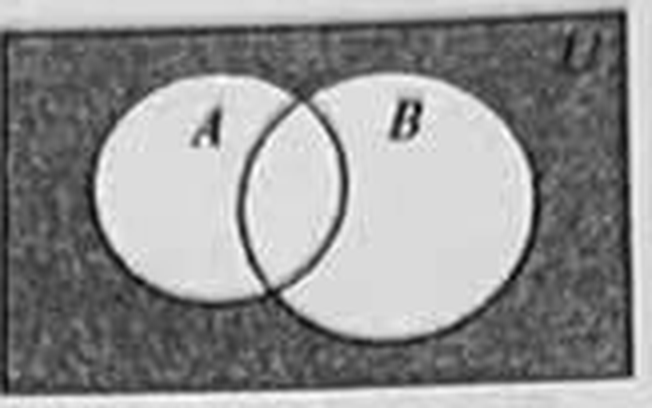
\includegraphics[width=0.30\textwidth]{figures/venn_AB_complement.png}
\end{center}
\mistakefields

\item 在集合 $U=\{a,b,c,d\}$ 的子集中选出 2 个不同的子集，需同时满足以下两个条件：(1)$a,b$ 都要选出 (2)对选出的任意两个子集 $A$ 和 $B$，必有 $A\subseteq B$ 或 $B\subseteq A$，那么共有 \blankline[2.4em] 种不同的选法.
\mistakefields

\item 设 $T$ 是由正三角形 $P_1P_2P_3$ 边上及其内部的点构成的集合，点 $O$ 是 $\triangle P_1P_2P_3$ 的中心. 若集合 $S=\{P\mid P\in T,\ |PO|\leqslant|PO_i|,\ i=1,2,3\}$，（符号 $|AB|$ 表示平面上两点 $A,B$ 间的距离），则集合 $S$ 表示的平面区域是\mbox{（\quad）.}

\keepwithprev
A. 四边形区域；\qquad B. 三角形区域；\qquad C. 六边形区域；\qquad D. 五边形区域；
\mistakefields

\item（10 分，第 1 小问 5 分，第 2 小问 5 分）已知 $A=\{x\mid x^2+x-2=0\}$，$B=\{x\mid x^2+ax+2a-4=0\}$.

\begin{enumerate}[label=(\arabic*)]
\item 若 $A=B$，求实数 $a$ 的值；
\item 若 $B\subseteq A$，求实数 $a$ 的值.
\end{enumerate}
\mistakefields

\item（11 分，第 1 小问 3 分，第 2 小问 3 分，第 3 小问 5 分）已知非空数集 $S$ 满足：对任意给定的 $x,y\in S$（$x,y$ 可以相同），有 $x+y\in S$ 且 $x-y\in S$.

\begin{enumerate}[label=(\arabic*)]
\item 哪个数一定是 $S$ 中的元素?说明理由；
\item 若 $S$ 是有限集，求 $S$；
\item 若 $S$ 中最小的正数为 5，求 $S$.
\end{enumerate}
\mistakefields

\item 已知集合 $A,B,C\subseteq\{1,2,3,\cdots,2024\}$，且 $A\subseteq B\subseteq C$，则有序集合组 $(A,B,C)$ 的个数是 \blankline[3.2em].
\mistakefields

\item 已知集合 $M=\{1,2,\cdots,10\}$，对它的非空子集 $A$，将 $A$ 中的每个元素 $k$ 都乘以 $(-1)^k$ 再求和，如 $A=\{2,3,6\}$，可求得和为 $(-1)^2\times 2+(-1)^3\times 3+(-1)^6\times 6=5$. 试对 $M$ 的所有非空子集，求这些和的总和 \blankline[3.2em].
\mistakefields

\item 设 $a_1,a_2,a_3,a_4$ 是 4 个有理数，使得 $\{a_ia_j\mid 1\leqslant i<j\leqslant 4\}=\left\{-24,-2,-\dfrac{3}{2},-\dfrac{1}{8},1,3\right\}$. 求 $a_1+a_2+a_3+a_4=$ \blankline[3.2em].
\mistakefields

\end{enumerate}

% ============================================================ 第三组
\bigsec{三、高一上数学第二周周末练习2（原错题 13--16）}

\begin{enumerate}[label=\textbf{原错题\arabic*.},leftmargin=*,itemsep=0.55em]
\setcounter{enumi}{12}

\item 若 $a,b$ 都是实数，试从 ①$a^3+8b^3=0$，②$a(|a|+|b|)=0$，③$a^2+b^2=0$ 中选出所有适合的条件，用序号填空：

\begin{enumerate}[label=(\arabic*)]
\item “$|a|+|b|=0$”的充要条件是 \blankline[2.4em]；
\item “$a+2b\geqslant 0$”的充分不必要条件是 \blankline[2.4em]；
\item “$a=0$ 且 $b=1$”的必要不充分条件是 \blankline[2.4em].
\end{enumerate}
\mistakefields

\item 从集合 $U=\{1,2,3,4,5,6,7,8,9,10\}$ 的子集中选出两个非空集合 $A,B$，同时满足以下两个条件：①$A\cup B=U$ 且 $A\cap B=\varnothing$；②若 $x\in A$，则 $x+1\in B$. 则共有 \blankline[3.2em] 种不同的选择.
\mistakefields

\item 已知集合 $A=\{x\mid -1<x<4\}$，$B=\{x\mid a-1\leqslant x\leqslant a+2\}$，若集合 $A\cap B$ 中恰好只有两个整数，则实数 $a$ 的取值范围是\mbox{（\quad）.}

\keepwithprev
A. $[-1,0)\cup(2,3]$\qquad B. $(-1,0)\cup(2,3)$\qquad C. $(-2,-1]\cup[3,4)$\qquad D. $(-2,-1)\cup(3,4)$
\mistakefields

\item 已知集合 $P=\{1,2,3,4,5\}$，若 $A,B$ 是 $P$ 的两个非空子集，则所有满足 $A$ 中的最大数小于 $B$ 中的最小数的集合对 $(A,B)$ 的个数为\mbox{（\quad）.}

\keepwithprev
A. $49$\qquad B. $48$\qquad C. $47$\qquad D. $46$
\mistakefields

\end{enumerate}

\end{document}
